%% LaTeX-Beamer template for KIT design
%% by Erik Burger, Christian Hammer
%% title picture by Klaus Krogmann
%%
%% version 2.0
%%
%% mostly compatible to KIT corporate design v2.0
%% http://intranet.kit.edu/gestaltungsrichtlinien.php
%%
%% Problems, bugs and comments to
%% burger@kit.edu

\documentclass[t,14pt,aspectratio=169]{beamer}
\usetheme{kit}
\usepackage[utf8]{inputenc}
\usepackage[babel, ngerman]{csquotes}
\usepackage{listings}
\usepackage{pgfpages}
%\setbeameroption{show notes on second screen}

\setbeamercovered{%
still covered={
	\opaqueness<1>{0}
}
}

%% TITLE PICTURE

% if a custom picture is to be used on the title page, copy it into the 'logos'
% directory, in the line below, replace 'mypicture' with the 
% filename (without extension) and uncomment the following line
% (picture proportions: 63 : 20, *.eps format if you use latex+dvips+ps2pdf,
% *.jpg/*.png/*.pdf if you use pdflatex)

\titleimage{title}

%% TITLE LOGO

% for a custom logo on the front page, copy your file into the 'logos'
% directory, insert the filename in the line below and uncomment it

\titlelogo{megi}

% (*.eps format if you use latex+dvips+ps2pdf,
% *.jpg/*.png/*.pdf if you use pdflatex)

%% BIBTEX ICON/KEY

% if you want to see BibTeX keys in the references view instead of the symbol,
% uncomment the following line
% \usebibitemtemplate{\insertbiblabel}

% the presentation starts here

\title{Peridiummmmm}
\subtitle{Eine Demo auf einem ARM-Mikrocontroller}
\author{ryx{\textasciicircum}SVatG, halcy{\textasciicircum}SVatG}

\begin{document}

% change the following line to "ngerman" for German style date and logos
% \selectlanguage{ngerman}

\date{June 9, 2012}

%title page
\begin{frame} % DUR: 0:00
\titlepage
\end{frame}

%table of contents -> NOPE
% \frame{
% \frametitle{Outline}
% \Large
% \tableofcontents
% }

\section{Foo}
\subsection{Bar}

\begin{frame} % DUR: 4:12
\frametitle{Die Platform}

\begin{minipage}{0.6\linewidth}
\begin{itemize}
\item Prozessor: Cortex M4, 168MHz, 192kB RAM
\item Audiohardware: Soundchip per I2S
\item Videohardware: 
\begin{itemize}
\item Portpins
\item 11 Widerstände
\item 1 VGA-Buchse
\item DMA
\end{itemize}
\item Kostenpunkt: ca. 17 EUR
\end{itemize}
\end{minipage}
\begin{minipage}{0.35\linewidth}
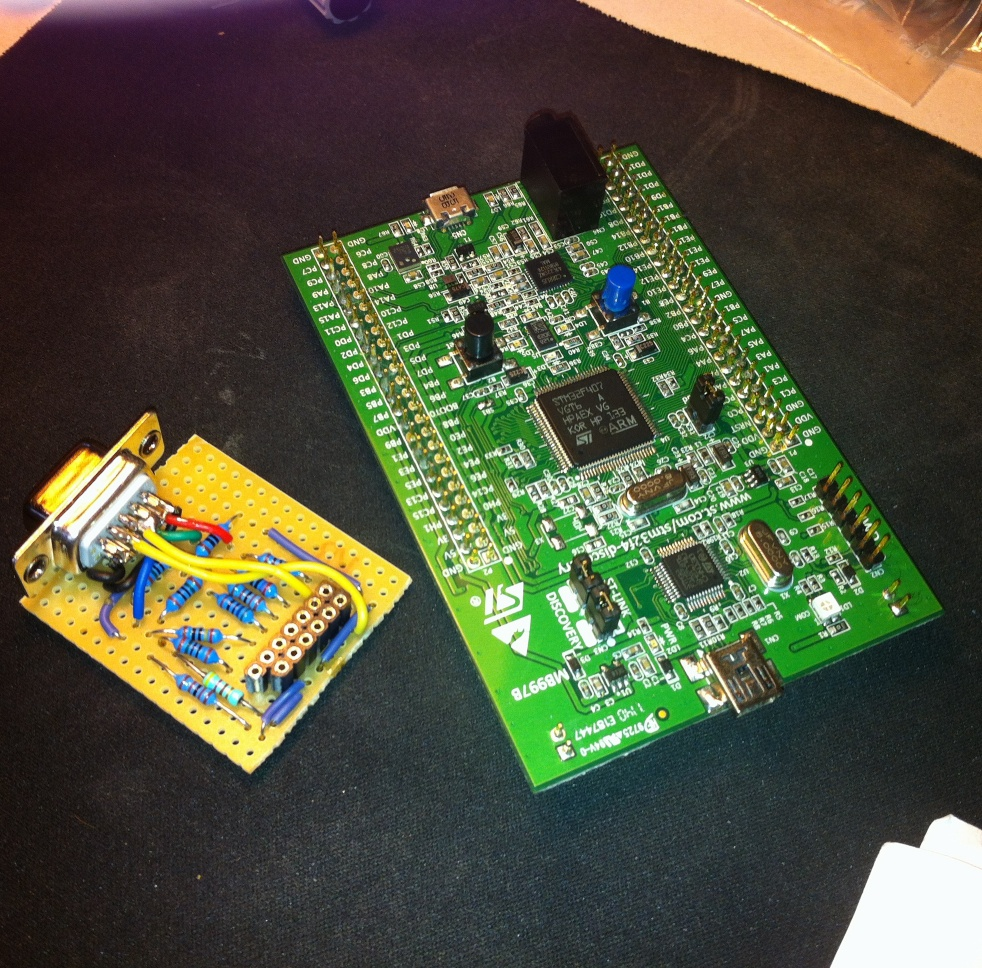
\includegraphics[width=\linewidth]{photos/cut}
\end{minipage}
\end{frame}


\end{document}
